\documentclass[10 pt]{article}
\usepackage{graphicx}
\pagestyle{plain}
\usepackage[OT4]{polski}
\usepackage[utf8]{inputenc}
\title{Sprawozdzanie 7 \\ \emph{\textbf{Grafy}}}
\author{Paweł Żurek 200404}
\date{30.04.2014}
\begin{document}
\tableofcontents
\maketitle
\section{Wstęp}
Prosty program, w którym użyte są podstawowe funkcje grafów.
\section{Krótki opis programu}
\textbf{Program po uruchomieniu pyta się z ilu wierzchołków ma stworzyć graf a następnie udostępnia proste menu : }
\begin{itemize}
\item Ustawienie połączeń między wierzchołkami
\item Dodanie wierzchołka
\item Usunięcie wierzchołka
\item Dodanie krawędzi
\item Usunięcie krawędzi
\item Wyświetlenie sąsiadów wierzchołka
\item Wyświetlenie grafu ( za pomocą macierzy połączeń )
\item Podanie ilości wierzchołków
\item Wyświetlenie aktualnych wierzchołków
\end{itemize}
Jako, że zaimplementowałem strukturę grafu za pomocą macierzy połączeń, najważniejszym elementem mojego programu jest : 
\begin{itemize}
\item Macierz typu int ( tablica dynamiczna dwu wymiarowa ) przechowująca aktualne połączenia między wierzchołkami
\end{itemize}
Oprócz tego niesamowicie ważna jest tablica typu int z aktualnymi wartościami wierzchołków. Jest potrzeba, ponieważ bez niej program nie działałby poprawnie po usunięciu chociaż jednego wierzchołka.\\
W programie jest zaimplementowana tablica typu string z wartościami wierzchołków, aczkolwiek na stan obecny ( 30.04.2014 ) jej nie używam.

\paragraph{Przykładowy wynik działania programu : }
\begin{center}
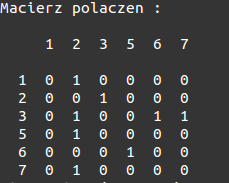
\includegraphics[scale=1]{wynik.png}
\end{center}

\section{Wnioski:}
\begin{itemize}
\item Program działa poprawnie
\item Macierz połączeń w prosty i jasny sposób ilustruje aktualny stan grafu
\item Dodawanie i usuwanie krawędzi w tej metodzie implementacji grafu jest bardzo proste, w przeciwieństwie do dodawania jak i usuwania wierzchołka
\end{itemize}


\end{document}